\section{Planning and Learning with Tabular Methods}
\subsection{Exercise 8.1}
\subsubsection{Q}
The nonplanning method looks particularly poor in Figure 8.3 because it is a one-step method; a method using multi-step bootstrapping would do better. Do you think one of the multi-step bootstrapping methods from Chapter 7 could do as well as the Dyna method? Explain why or why not.
\subsubsection{A}
If we used a multi-step bootstrapping method (e.g. n-step Sarsa), we could back-propogate the reward from the final timestep along the trajectory followed for some large value of $n$. This of course would only update the action-values of the $n$ action-values prior to receiving the reward and leave the remain 1700 - $n$ action values unchanged. When running a second episode using this approach, the agent would still act naively until it reached its first state-action pair with some value, which it could then bootstrap from to update previous states. Without a model of the environment (like Dyna) it cannot plan in the same way, and cannot reap the efficiency gains that Dyna enjoys. 

$
\hfill \blacksquare
$

\subsection{Exercise 8.2}
\subsubsection{Q}
Why did the Dyna agent with exploration bonus, Dyna-Q+, perform better in the first phase as well as in the second phase of the blocking and shortcut experiments?
\subsubsection{A}
I'm not sure it is performing \textit{better}, rather that the Dyna-Q+ algorithm is increasing the reward associated with every state at every timestep when Dyna-Q is not, so cumulative reward must be higher in absolute terms than Dyna-Q. In this sense a direct comparison on the basis of cumulative reward is perhaps unfair. Due to the increased exploration of the Dyna-Q+ algorithm, it is however likely that it found the optimal policy more quickly than Dyna-Q and so was able to exploit it quicker for higher cumulative reward

$
\hfill \blacksquare
$

\subsection{Exercise 8.3}
\subsubsection{Q}
Careful inspection of Figure 8.5 reveals that the difference between Dyna-Q+ and Dyna-Q narrowed slightly over the first part of the experiment. What is the reason for this?
\subsubsection{A}
Dyna-Q+ is forced to explore continually having already obtained the optimal policy, meaning that when Dyna-Q is exploiting its learned optimal policy, Dyna-Q+ is exploring sub-optimal trajectories and receiving less reward.

\subsection{Exercise 8.4}
\subsubsection{Q}
The exploration bonus described above actually changes the estimated values of states and actions. Is this necessary? Suppose the bonus $k\sqrt{\tau}$ was used not in updates, but solely in action selection. That is, suppose the action selected was always that for which $Q(S_t, a) + k\sqrt{\tau(S_t, a)}$ was maximal. Carry out a gridworld experiment that tests and illustrates the strengths and weaknesses of this alternate approach.
\subsubsection{A}
\ProgrammingExercise \\
\begin{figure}[h!]
	\centering
	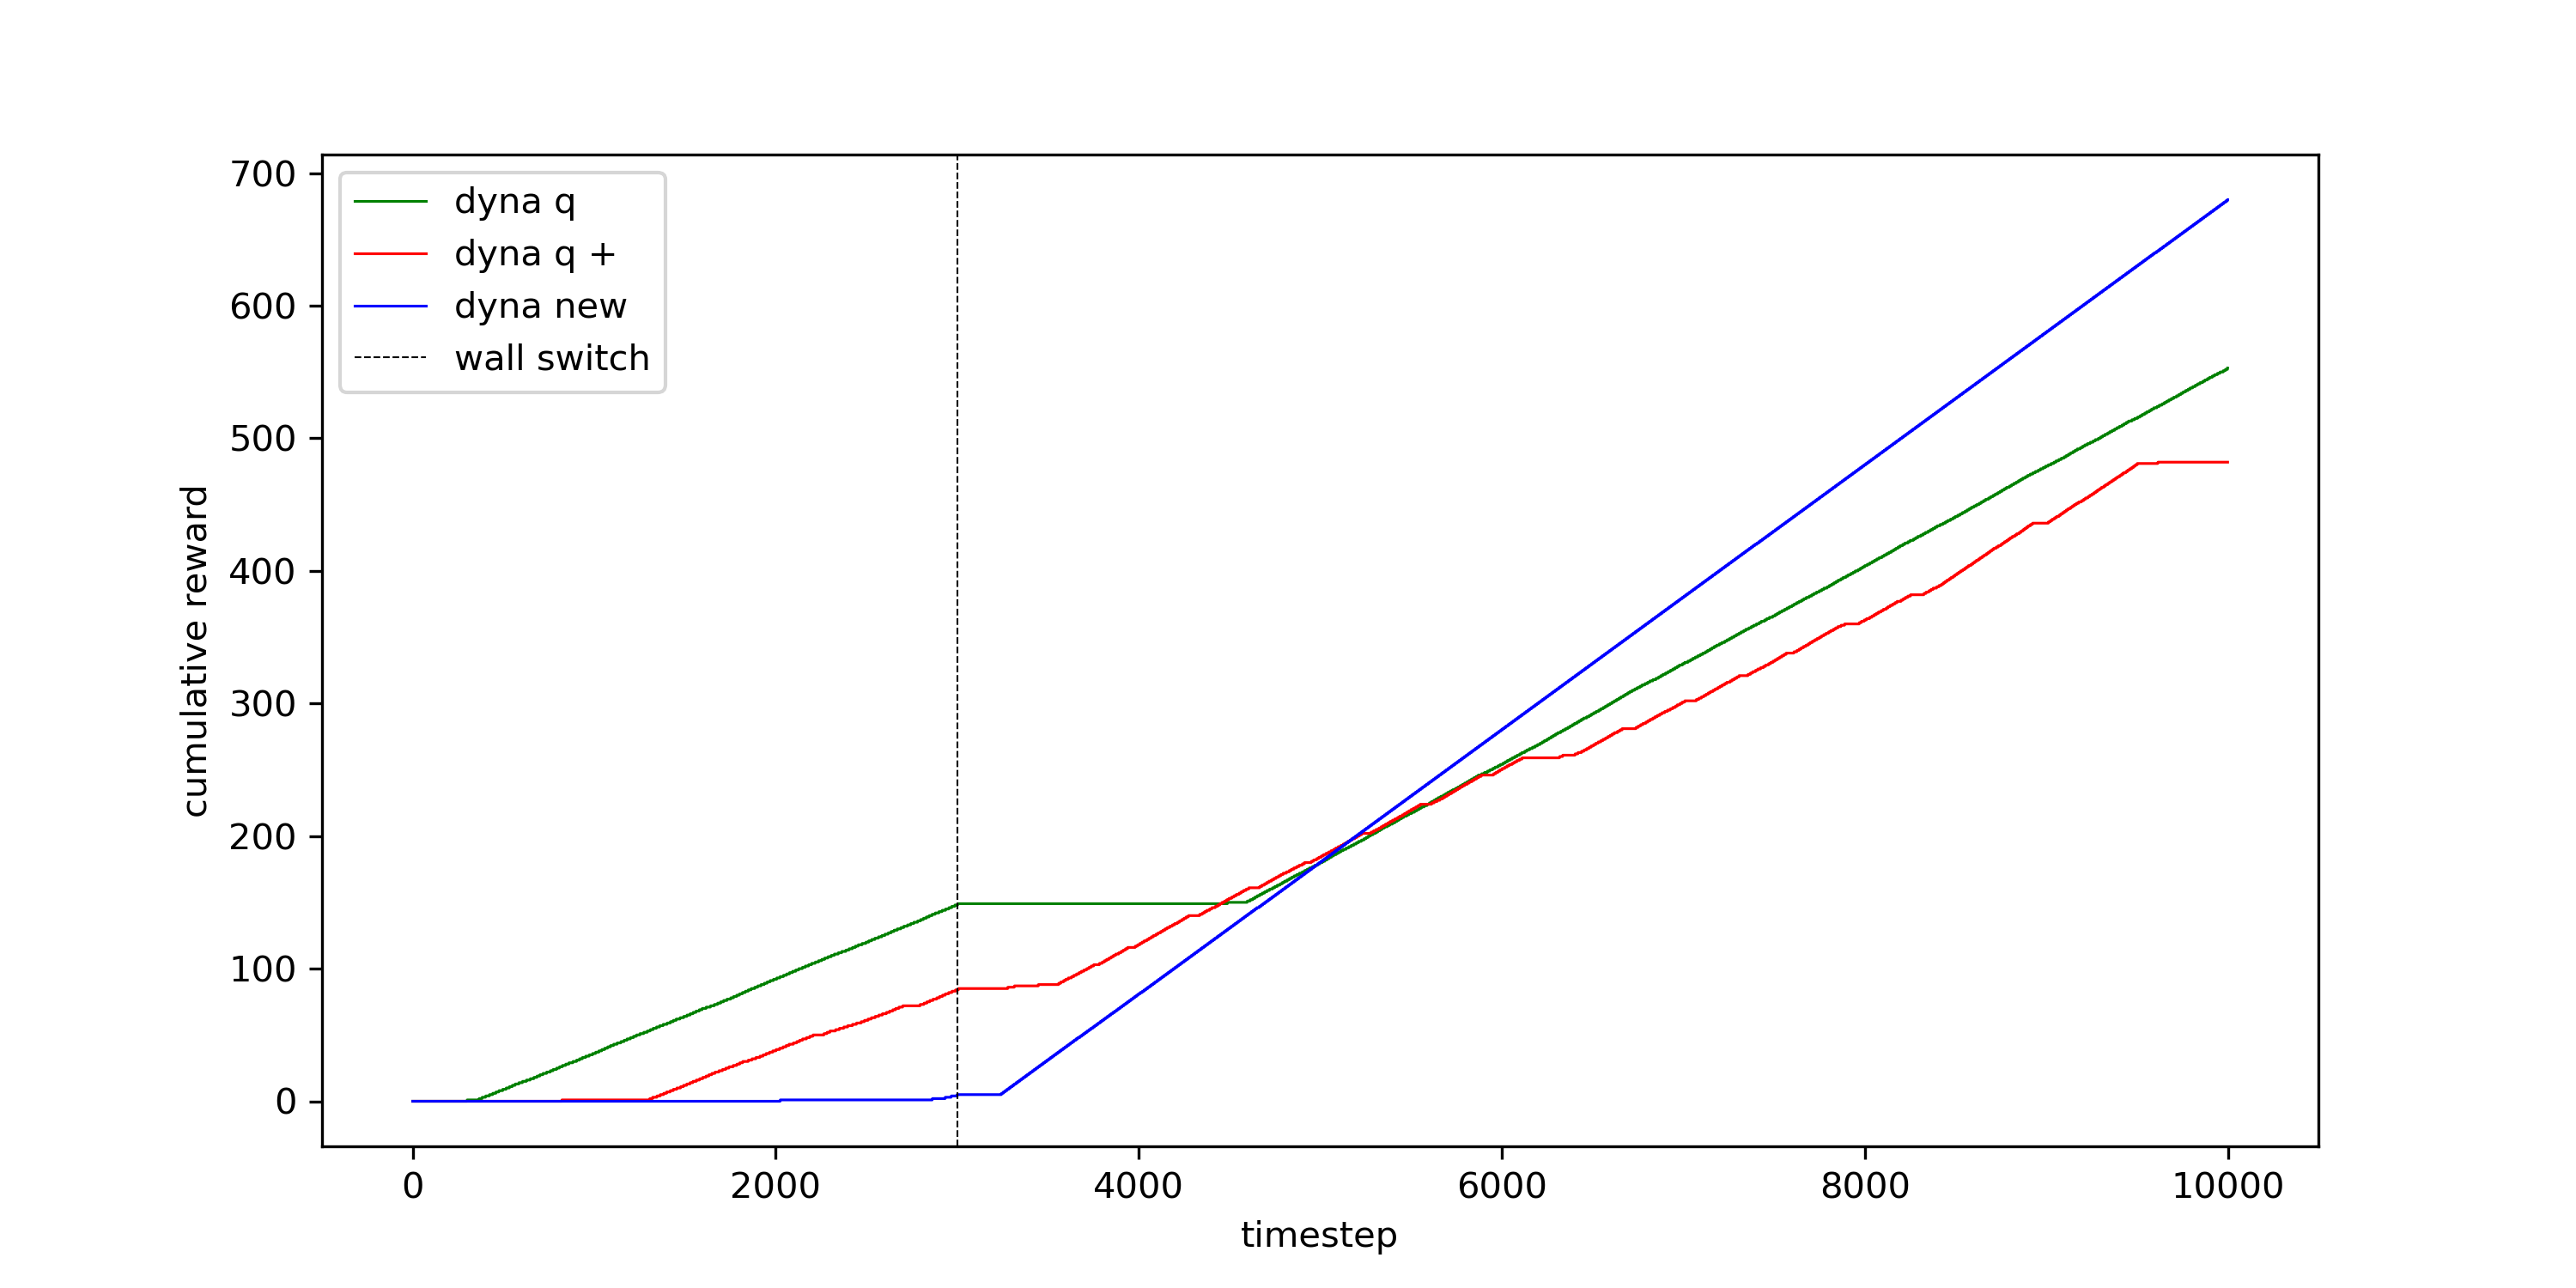
\includegraphics[width=\textwidth]{/ex8.4}
	\caption{Cumulative reward for three model-based agents on the blocked maze task after 10000 timesteps}
	\label{fig: 8.4}
\end{figure}

\subsection{Exercise 8.5}
\subsubsection{Q}
How might the tabular Dyna-Q algorithm shown on page 164 be modified to handle stochastic environments? How might this modification perform poorly on changing environments such as considered in this section? How could the algorithm be modified to handle stochastic environments \textit{and} changing environments?
\subsubsection{A}
\begin{figure}[h!]
	\centering
	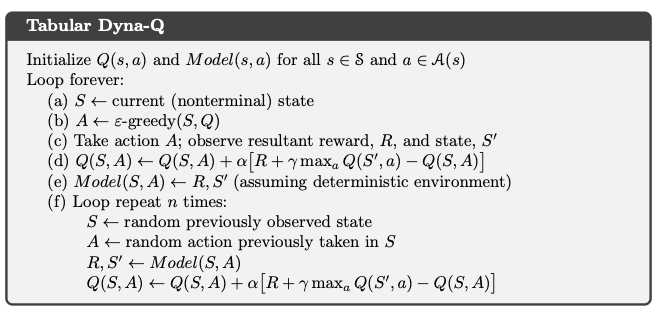
\includegraphics[width=\textwidth]{/ex8.5}
	\caption{Tabular Dyna-Q algorithm}
	\label{fig: dyna-Q}
\end{figure}
\begin{itemize}
\item In part (e) of the algorithm, instead of updating $R$ and $S'$ directly, we would store samples of $R$ and $S'$ from which we can compute distributions and thus expectations. 
\item This would perform poorly because it would be bias toward earlier observations made in the unchanged environment.
\item We could likely rectify this by weighting more recent observations, or discounting past observations in the distribution. Equally we could quantify the agent's confidence in its model e.g. if it hasn't selected a state-action pair in a long time, its confidence in its model should be low and vice versa. This could manifest as a relationship with $\tau$ as discussed with Dyna-Q+.
\end{itemize}